%%%%%%%%%%%%
\thispagestyle{empty}
\epigraph{ 
``\emph{
Ár var alda, \\
þar er Ýmir byggði, \\
var-a sandur n sær \\
n svalar unnir; \\
jörð fannst æva \\
n upphiminn, \\
gap var Ginnunga \\
en gras hvergi.}
''}{3rd verse of Völuspá}
\chapter{Introduction}
\label{ch:intro}

\epigraph{``\emph{
Þá gengu regin öll \\
á rökstóla, \\
ginnheilög goð, \\
og um það gættust; \\
nótt og niðjum \\
nöfn um gáfu, \\ 
morgun htu \\
og miðjan dag, \\
undorn og aftan, \\
árum að telja.} 
''}{6th verse of Völuspá}


There is strong observational evidence that extremely compact and massive objects populate the Universe, these objects are commonly referred to as \textit{black holes}.
According to the paradigm of general relativity, black holes are extremely constrained objects, which are effectively described by the Kerr metric when near equilibrium, which depends solely on two parameters.
This idea, partly based on rigorous mathematical theorems, but partly conjectured, has been immortalized in John Wheeler's mantra ``\textit{black holes have no hair}''~\cite{Misner:1974qy}. 


In this first chapter, after a review of the observational evidence for black holes and the general relativity black hole paradigm, we shall look into the limitations of the ``no-hair'' idea.
Some of these have been known for some time, but we shall focus on a recently discovered case: ``Kerr black holes with scalar hair''.
To describe these new solutions, we will need to briefly review a particular type of gravitating solitons called \textit{boson stars}, as well as the phenomenon of \textit{superradiance} known to occur in the Kerr spacetime.
   
\section{Observational evidence for extremely compact objects}

At the center of our galaxy resides an object known as Sagittarius A$^\star$.
From the orbits of stars in its vicinity, its mass has been estimated as $4.1\times 10^6$ M$_\odot$ (where M$_\odot$= 1 solar mass)~\cite{Ghez:2008ms}.
From the orbit with the smallest pericenter, a size constraint of $17$ light hours has been placed on the object, and this upper bound can be further refined to about $6$ light hours by using other observations~\cite{Ghez:2003qj}.
The only known theoretical candidate from well established physical models which fits these observational data is a \textit{black hole}.
Thus Sagittarius A$^\star$, as well as other similar compact objects at the center of other galaxies, is commonly referred to as a \emph{supermassive black hole}.
Black hole candidates of this type have been found in a mass range between $10^6$ and $10^{10}$ M$_\odot$~\cite{Narayan:2013gca} and they play a central role in both the formation and growth of their host galaxies \cite{Kormendy:2013pja} so understanding them is of vital importance for the models of structure formation in the Universe.

Another case of extremely compact and massive objects is found in binary systems in our galaxy, where strong X-ray sources exist.
One example of such an object is Cygnus X-1, known since the 1960s~\cite{1965Sci...147..394B}.
Using methods which have been used for over a century on ordinary stars in binary systems, the estimated masses of these $24$ binaries were found to range between $5$ and $30$ M$_\odot$~\cite{Narayan:2013gca}.
For example, Cygnus X-1 has an estimated mass of 14.8 M$_\odot$~\cite{Reid:2011nn}.
\textit{Neutron stars}, as the most compact directly observable objects currently known, have masses which are below $3$ M$_\odot$ \cite{Kalogera:1996ci,Rhoades:1974fn}.
Therefore, these X-ray sources are in all likelihood black holes and due to their mass range, have been called \textit{stellar mass black holes}.

The objects discussed in the previous two paragraphs are strictly speaking only black holes candidates, 
as there might be some, as of yet unknown, form of matter which they could be made of, making what is generically referred to as a \textit{black hole mimicker}.
On the other hand, if these objects are black holes, one should ask whether they are the paradigmatical black holes of general relativity, to be discussed in Sec. \ref{sec:bh_gr}, or black holes as described by some alternative model.
The next decade promises to shed light on both of these issues: we are on the verge of gathering observational evidence that will map the spacetime geometry close to these black hole candidates.
This evidence will be obtained by both gravitational wave astronomy~\cite{Hild:2011np,Hobbs:2009yy,Seoane:2013qna} and by large baseline interferometry measurements of the galactic center, using the Event Horizon Telescope (EHT).
The latter, promises to resolve angular scales of the order of the horizon scale for the Sagittarius A$^\star$ black hole candidate~\cite{Loeb:2013lfa}.
The EHT will study the so-called black hole \textit{shadows}~\cite{Falcke:1999pj}: the gravitational lensing effect due to the black hole on the radiation from background sources, with respect to the observer.

These forthcoming experiments make it particularly timely to explore alternative models to the general relativity black hole paradigm, and their associated phenomenology.
But before we dwell on these alternative models, let us first review the standard paradigm.
\section{The general relativity black hole paradigm}
\label{sec:bh_gr}

In physical terms, a black hole is a region of spacetime from which nothing can escape.
The boundary of this region is known as the \textit{event horizon}.
More technically, a black hole is a solution to Einstein's general relativity (or some generalization thereof) possessing an event horizon.
In the case of general relativity one solves the field equations,
\begin{align}
  R_{ab} - \frac{1}{2}g_{ab}R  &= 8\pi T_{ab},
  \label{eqn:Einstein-eqns}
\end{align}
where $R_{ab}$ is the Ricci tensor, $R$ the Ricci scalar, $T_{ab}$ the stress-energy tensor and $g_{ab}$ the metric tensor.
Here and throughout this thesis we will use geometrized units, with $G=1=c$.

The black hole solutions we will start by considering are both stationary, i.e. equilibrium states, and electrovacuum.
That is, there exists an asymptotically timelike Killing vector field in the spacetime and the only matter-energy content present are electromagnetic fields.
Surprisingly, and in sharp contrast to stars, equilibrium black hole solutions in this theory can be completely described by only three parameters: their mass, angular momentum and electric charge~\cite{Chrusciel:2012jk}.
These parameters are defined by the gravitational and electromagnetic fields far away from the black hole, since they have associated Gauss laws.
In this section, we will further restrict ourselves mainly to uncharged black holes, as it is generally believed that astrophysically relevant black holes will be essentially electrically neutral, due to efficient discharging mechanisms.
What remains is a 2-parameter family, where the two parameters are the mass, $M$, and angular momentum, $J$, described by the \textit{Kerr metric} \cite{Kerr:1963ud}, named after Roy Kerr, who discovered this solution in 1963.
We shall now describe some properties of this important geometry.

In order for the Kerr spacetime to have an event horizon, the angular momentum per unit mass has an upper bound given by the mass of the black hole: $J/M\le M$.
When the angular momentum goes to zero, one obtains the non-rotating Schwarzschild black hole, while at its upper limit, one obtains the single-horizon extremal Kerr solution.
For values between these two limiting cases, the Kerr black hole has two horizons, of which the outer one is the event horizon.
Kerr black holes also posses an ergoregion where the time translation Killing vector field becomes spacelike outside the event horizon.
Within this region, observers can no longer counter rotate around the black hole.

The extraordinary importance of the Kerr metric was established in the early 1970s by the so-called \textit{black hole uniqueness theorems} \cite{Robinson:2004zz}.
These theorems, established originally for Einstein-Maxwell theory, state that the most general asymptotically flat stationary, axi-symmetric vacuum spacetime that is non-singular on and outside an event horizon, is a member of the Kerr-Newman family of solutions, a charged generalization of the Kerr solution.
In particular, in vacuum, the most general black hole solution is described by the Kerr metric.
This result showed that within Einstein-Maxwell theory black holes are very special, restricted objects, and \textit{suggested} this would remain the case even if more generic types of matter are included.
This led to the \textit{no-hair idea} or conjecture: that regardless of the type of matter available, the end state of gravitational collapse is a Kerr-Newman (to allow for electric charge, $Q$) black hole, solely characterized by $M$, $J$ and $Q$, all of which are conserved quantities subject to a Gauss law, and no additional degrees of freedom, to which \textit{hair} provides a metaphor, are needed.
Together, the uniqueness theorems, and the no-hair conjecture, built the general relativity black hole paradigm: that the millions of stellar mass black holes and the one supermassive black hole in \textit{each} galaxy, are all, when near equilibrium, described by the Kerr metric.  

We emphasize that an important distinction has to be made between the uniqueness theorems and the no-hair conjecture.
The uniqueness theorems hold for Einstein-Maxwell theory and have been mathematically proven, while the no-hair conjecture is a more generic idea that has only been proven for a limited set of models (see e.g.~\cite{Bekenstein:1996pn}).
In fact, as we shall now discuss, examples have long been known to exist which violate the no-hair idea, at least in its most strict sense.
\section{Beyond the conventional: hairy black holes}
\label{sec:bh_beyond_gr}

One of the simplest types of ``matter'' often considered by physicists is provided by \textit{scalar fields}.
Since 2012, there is observational evidence that scalar fields exist in nature, by virtue of the discovery of a scalar particle at the Large Hadron Collider, at CERN, tentatively identified with the standard model Higgs boson~\cite{Aad:2012tfa,Chatrchyan:2012ufa}.
But for decades, scalar fields have been considered in phenomenological models, in particular within gravitational physics.
A notable example is cosmology, where various types of scalar fields have been used to model dark energy and dark matter.
One reason is that scalar fields are well motivated by some high energy physics models such as string theory.
Yet another reason is that scalar fields may be considered as a proxy to realistic matter, such as perfect fluids.

It is therefore quite natural that in testing the no-hair idea, scalar fields were one of the first types of ``matter'' considered.
This program was initiated by Chase~\cite{Chase:1970wq} who established that ``every zero-mass scalar field which is gravitationally coupled, static and asymptotically flat, becomes singular at a simply-connected event horizon''.
In other words, a black hole spacetime cannot support a regular massless scalar field in equilibrium with it; i.e. no \textit{black hole (massless) scalar hair}.
Further ``no-scalar-hair'' theorems were developed by Bekenstein~\cite{Bekenstein:1971hc,Bekenstein:1972ky} who also considered massive scalar, vector and spin 2 fields (see also the review~\cite{Bekenstein:1996pn}) and Hawking~\cite{Hawking:1972qk}, who showed that in the Brans-Dicke theory of gravity~\cite{Brans:1961sx}, in which there is a scalar field non-minimally coupled to the geometry, the regular black hole solutions are the same as in general relativity.
Hawking's theorem was then generalized~\cite{Sotiriou:2011dz} to more general \textit{scalar-tensor theories of gravity}, of which the Brans-Dicke model is an early example.

A few remarks are in order concerning ``no-scalar-hair'' results for black holes.
First of all, we are focusing on regular configurations.
Solutions where the scalar field diverges at the horizon are known (see e.g.~\cite{BBM}), but they appear to have no physical relevance.
We are also considering independent scalar fields.
Considering \textit{simultaneously} gauge fields to which the scalar fields are non-minimally coupled leads to solutions~\cite{Gibbons:1982ih,Gibbons:1987ps} - notably $p$-brane type solutions in supergravity~\cite{Horowitz:1991cd}; but these have no independent scalar charge and the scalar field vanishes when the electromagnetic field vanishes.
Finally, we are focusing on four dimensional, asymptotically flat black holes.
Considering, for instance, Anti-de-Sitter asymptotics can allow for hairy black holes, since the asymptotic nature of the spacetime yields a trapping mechanism from which the scalar field cannot escape. 

It turned out that progress in finding regular hairy black holes came from a different direction: the study of \textit{gravitating solitons}.
These are self-gravitating, horizonless, regular configurations, which are found in Einstein gravity coupled to (typically) non-linear matter sources.
An influential pioneering example was the Bartnik-Mckinnon ``particle-like'' solution of the Einstein-Yang-Mills equations~\cite{Bartnik:1988am}.
That a black hole could be added at the center of these solitons was found first by Volkov and Galtsov~\cite{Volkov:1989fi}, and later by Bizon~\cite{Bizon:1990sr}, yielding \textit{black holes with Yang-Mills hair} also dubbed \textit{colored black holes}.
Other examples along similar paths were obtained with other non-Abelian gauge fields (e.g. \cite{Droz:1991cx,Lavrelashvili:1992cp}; see also the reviews~\cite{Bizon:1994dh,Volkov:1998cc}).

The intuitive, physical reason for why the solutions in the previous paragraph exist comes about from a balance between the non-Abelian gauge-field repulsion and the gravitational attraction.
This kind of balance between two competing effects, to keep the hair in equilibrium in the vicinity of the black hole, seems to be vital for the existence of all types of hairy black hole solutions.
These examples, moreover, serve to show the \textit{mathematical} limitations of the no-hair idea.
They seem, however, of limited astrophysical relevance since it is not expected that, say, Yang-Mills fields, play an important role in macroscopic astrophysical black holes.
Moreover, some of these solutions (but not all) are  either unstable and/or do not introduce a new quantity that characterizes the black hole \cite{Mavromatos:1995fc}.

The hairy black holes we have described occur in theories that also admit gravitating solitons. This gave rise to a suggestion that hairy black holes could be regarded as bound states of ``conventional paradigm'' black holes with gravitating solitons~\cite{Ashtekar:2000nx}. But an intriguing exception to this picture was known involving, precisely, a type of self-gravitating soliton made out of a scalar field: \textit{boson stars}, which we shall now describe.





\section{Boson stars}
\label{sec:bs}
Boson stars are self-gravitating, regular, asymptotically flat, complex scalar fields, first discussed by Kaup~\cite{Kaup:1968zz} and Ruffini and Bonazzola~\cite{Ruffini:1969qy} in the late 1960s (see~\cite{Schunck:2003kk} for a review).
The simplest boson stars are solutions of Einstein's gravity minimally coupled to a complex massive scalar field, $\Psi$, i.e. \textit{Einstein-(massive)-Klein-Gordon theory}, described by the action
\begin{equation}
\mathcal{S}= \int  d^4x\sqrt{-g}\left[\frac{R }{16\pi }
   - g^{ab}\Psi_{, \, a}^* \Psi_{, \, b} - \mu^2 \Psi^*\Psi
 \right] \ ,
 \label{Introaction}
 \end{equation}
where $\mu$ is the scalar field mass.
Other models are obtained by replacing the mass term in \eqref{Introaction} by a more complicated self-interaction potential for the scalar field. 

One distinctive feature of boson stars, as compared to other gravitating solitons, is that the scalar field is \textit{time-dependent}: $\Psi(t,{\bf x})=e^{-iwt}\phi({\bf x})$, where ${\bf x}$ are the spatial coordinates and $w$ is the scalar field's frequency.
This phase-like time dependence, however, vanishes at the level of the energy momentum tensor, $T_{ab}=2 \Psi_{ , (a}^*\Psi_{,b)}-g_{ab}  [  \Psi_{,c}^*\Psi^{,c}+\mu^2 \Psi^*\Psi]$, even though an imprint of $w$ remains, thus making it possible to source a \textit{time-independent} geometry.
As such, the geometry of boson stars admits a (at least asymptotically) timelike Killing vector field and may be regarded as a stationary configuration. 

Both spherically-symmetric as well as axially-symmetric, i.e. rotating, boson star solutions are known, but only as numerical solutions -- no known closed form analytic solution has been found.
Here we shall focus on the rotating case. 

Rotating boson stars were first discussed by Yoshida and Eriguchi~\cite{Yoshida:1997qf} and Schunk and Mielke~\cite{Schunck:1996he}.
A convenient parameterization of the metric is given below (cf. eq. \eqref{eqn:HBH-ansatz}, with $r_H=0$).
The metric ansatz therefore introduces four real functions of $(r,\theta)$.
The scalar field ansatz is of the form, 
\begin{align}
  \Psi &= \phi(r,\theta)e^{i(m\varphi-w t)},
  \label{eqn:field-ansatz}
\end{align}
and thus introduces a fifth real function which describes the field's angular and radial profile.
It also introduces an azimuthal harmonic index $m\in \mathbb{Z}^\pm$.
Each value of $m$ labels a sub-family of boson star solutions.
Finally, the solutions are labelled by yet another discrete number $n\in \mathbb{N}_0$, which counts the number of nodes of the scalar field profile.
Solutions with $n=0$ are regarded as fundamental states (for each $m$) and solutions with $n>0$ as excited states and throughout this thesis, we will only consider $n=0$ solutions.
To summarize, rotating boson stars are described by five functions of $(r,\theta)$, which are determined after fixing two integers $n,m$ and one continuous parameter $w$.
The solutions are obtained solving five non-linear, coupled partial differential equations, with appropriate boundary conditions.
It turns out that solutions only exist in a range certain frequency range between $w=\mu$ and some minimal frequency $w_{min}$ (cf. Fig. \ref{fig:HBH-parameter-space}).

An observation that will become relevant in the following is that, although the line element~\eqref{eqn:HBH-ansatz} admits two Killing vector fields, $\partial_t$ and $\partial_\varphi$, the full solution, including the scalar field \eqref{eqn:field-ansatz} is only preserved by a single, helicoidal Killing vector field of the form
\begin{equation}
k=\partial_t+\frac{w}{m}\partial_\varphi \ . 
\label{kvf}
\end{equation}

Unlike the gravitating solitons discussed in Sec. \ref{sec:bh_beyond_gr}, it was not known, until recently, if a black hole could be added at the center of a boson star.
The investigation of this question would turn out to unveil a new type of hairy black holes, that will be discussed in Sec. \ref{sec:HBHs}.
But before that, we need to survey a particular property of Kerr black holes. 
\section{Superradiance of Kerr black holes}

Kerr black holes can amplify scalar (and other types of bosonic) waves.
This phenomenon is called \textit {superradiant scattering}~\cite{Misner:1972kx} (following the work on the analogous particle like phenomenon in~\cite{Penrose:1969pc,Christodoulou:1970wf}).
This has been shown to occur if the frequency of an ingoing monochromatic wave -- with a temporal and azimuthal dependence of type \eqref{eqn:field-ansatz} -- satisfies the condition 
\begin{equation}
w<m\Omega_H \ , 
\label{super_cond}
\end{equation}
where $\Omega_H$ is the angular velocity of the outer black hole horizon~\cite{Bardeen:1972fi,Starobinsky:1973a,Press:1972zz}.
During this scattering process, energy is extracted from the black hole in a way consistent with the second law of black hole dynamics~\cite{Bardeen:1973gs}, i.e. the area of the black hole does not decrease.
Therefore, it is only rotational energy that is being extracted from the black hole.

If there is a trapping mechanism present, which confines the field in the vicinity of the black hole, a \textit{superradiant instability} occurs, since the field is recurrently scattered and amplified, triggering a potentially explosive phenomenon, some times called a \textit{black hole bomb}~\cite{Press:1972zz}. 
A massive field or a timelike asymptotic (conformal) boundary provide two examples of natural trapping mechanisms while a more ad hoc example is to impose a mirror-like boundary condition for the field at a finite distance from the horizon.
The superradiant instability has been studied in depth in recent years, mostly at the linear level (see e.g. \cite{Dolan:2007mj,Dolan:2012yt} and \cite{Cardoso:2013krh} for a review); fully non-linear studies, in which the backreaction of the field's amplification is taken into account on the geometry, are still under development~\cite{Okawa:2014nda,East:2013mfa}.
Consequently the end-state of the instability is still an open question.

As a side note, let us remark that for non-rotating but electrically charged black holes, it is possible to obtain superradiant scattering as long as the field itself possesses an electric charge~\cite{Bekenstein:1973mi}.
However, superradiant instabilities do not occur even if the field is massive in asymptotically flat spaces~\cite{Hod:2013eea,Hod:2013nn}, whereas they do in asymptotically Anti-de-Sitter spaces (see e.g.~\cite{Wang:2014eha}).
But in the former case the instability can be triggered by imposing a mirror-like boundary condition for the field\cite{Herdeiro:2013pia,Hod:2013fvl,Degollado:2013bha}.
This may be regarded as a toy model for the astrophysically more relevant rotating case, but it turns out to have both quantitative and qualitative differences when compared to the latter.  
For this toy model, a recent study showed that a hairy black hole solution is obtained dynamically from the instability\cite{Sanchis-Gual:2015lje}.

At the threshold of the instability, i.e. considering field modes with $\omega=m\Omega_H$, \textit{true stationary bound states} (in the sense of quantum mechanics) can exist, as there is neither decay nor growth of the field.
Even though considerable literature exists about superradiance, only recently these test field, stationary bound states have been studied in detail, and dubbed (in the scalar field case) \textit{scalar clouds around Kerr black holes}~\cite{Hod:2012px,Hod:2013zza,Herdeiro:2014goa}.
These configuration form a discrete set of solutions labelled by $3$ numbers, $(n,\ell,m)$, where $n$ corresponds to the node number of the radial part of the ``wave function'' in \eqref{eqn:field-ansatz} and $\ell$ and $m$ are the quantum numbers of the spheroidal harmonics that are used to separate the Klein-Gordon equation in the Kerr background (see e.g.~\cite{Brill:1972xj}).
It turns out that a given cloud, specified by a set $(n,m,l)$, does not exist for any Kerr background.
A quantization condition exists for the background parameters implying that a given cloud only exists along a $1$-dimensional \textit{existence line} of the $2$-dimensional Kerr parameter space.
This is illustrated in Fig. \ref{fig:clouds}, where a few existence lines are plotted (in dotted blue) in a mass (M) vs. horizon angular velocity ($\Omega_H$) diagram -- both in units of the scalar field mass $\mu$ -- for Kerr black holes. 
%
\begin{figure}[H]
  \begin{center}
  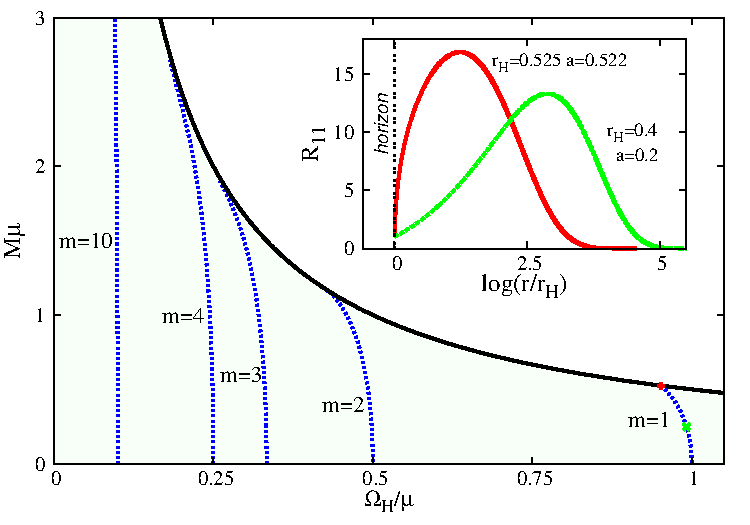
\includegraphics[height=2.78in]{Figs/unstable-OmegaH-M-clouds.pdf}
  \end{center}
  \caption{(Large plot) Mass vs. angular velocity diagram for Kerr black holes. Extremal black holes exist along the black solid line and other Kerr black holes below that line. A few existence lines for scalar clouds are plotted for $n=0$ and for different values of $l=m$ (blue dotted lines). (Inset) Two radial profiles of two particular clouds with $m=1=l$. The clouds are non-zero at the horizon, reach a maximum value at some radial distance and, asymptotically, decrease to zero exponentially. From Ref.~\cite{Herdeiro:2014goa}.}
  \label{fig:clouds}
\end{figure}

Thus, the existence of superradiance admits the existence of bound state solutions (clouds) which are zero modes of this instability.
In the next section we will describe how the backreaction of these clouds on the geometry leads to new black holes with scalar hair.

\section{A new type of hairy black holes}
\label{sec:HBHs}
The scalar clouds described in the previous section suggest that \textit{asymptotically flat rotating black holes with complex scalar hair} could exist.
Such solutions were indeed found in~\cite{Herdeiro:2014goa}, corresponding to a $5$-parameter family of solutions of the Einstein-(massive)-Klein-Gordon theory as described by \eqref{Introaction}.
Three of the parameters are continuous: the ADM mass, $M$, the ADM angular momentum, $J$, and a Noether charge, $Q$.
The last one is obtained by integrating the time component of the scalar field $4$-current on a spacelike slice and may be regarded as measuring the amount of scalar hair outside the horizon.
It is convenient to introduce a normalized Noether charge $q\equiv Q/2J$; then, $q$ is a compact parameter in the full space of solutions: $0\le q\le 1$.
The value $q=0$ corresponds to Kerr black holes, showing that these hairy black holes are continuously connected to the standard Kerr family, while for $q=1$ rotating boson stars are recovered, which obey $Q=2J$.
The solutions in~\cite{Herdeiro:2014goa} were dubbed \textit{Kerr black holes with scalar hair}.
The two remaining parameters of the solutions found in~\cite{Herdeiro:2014goa} are discrete and have already been described for boson stars: the azimuthal harmonic index $m\in \mathbb{Z}^\pm$ and the node number $n\in \mathbb{N}_0$. 

The hairy black hole solutions were found numerically using a metric ansatz of the form
\begin{align}
  ds^2 &= e^{2F_1}\left( \frac{dr^2}{N} + r^2d\theta^2 \right) + e^{2F_2}r^2\sin^2\theta \left( d\varphi - Wdt \right)^2 - e^{F_0}Ndt^2,
  \label{eqn:HBH-ansatz}
\end{align}
with $N\equiv 1-r_H/r$, and where $F_0,~F_1,~F_2,~W$ are functions of $r$ and $\theta$ only.
$r_H$ is the position of the event horizon of the black hole in this coordinate system.
We remark these are \textit{not} Boyer-Lindquist coordinates in the Kerr limit. 

In~\cite{Herdeiro:2014goa} the parameter and phase space for the solutions with $n=0$, $m=1$ were discussed in detail -- see Fig. \ref{fig:HBH-parameter-space}.
Here are some other salient features concerning these solutions.
There is a region of overlap of hairy and Kerr black holes with the same $M,J$ and in that sense there is non-uniqueness.
This degeneracy is raised by the introduction of $q$, i.e. no two solutions share the same set of $M,J,q$.
Some of these hairy black solutions violate the Kerr bound: $J\le M^2$.
This is not surprising since this is known to occur for rotating boson stars~\cite{Ryan:1996nk}, and hairy black holes are continuously connected to these stars.
It is indeed a generic feature that hairy black holes are more \textit{star-like} than Kerr black holes, i.e. less tightly constrained in their physical properties than Kerr black holes.
This observation has also implications for possible astrophysical phenomenology of these hairy black holes.
It was observed in~\cite{Herdeiro:2014goa} that both the quadrupole moment and the angular frequency at the innermost stable circular orbit (ISCO) can differ significantly for hairy black holes, as compared to the standard Kerr values.
Finally, hairy black holes have a richer structure of ergo-regions than Kerr, with the occurrence of \textit{ergo-Saturns}, besides ergo-spheres, in a region of parameter space~\cite{Herdeiro:2014jaa}.

\begin{figure}[H]
  \begin{center}
  \includegraphics[height=2.78in]{Figs/BH-w-M.pdf}
 %   \includegraphics[width=\textwidth]{BH-w-M.pdf}
  \end{center}
  \caption{(Large plot) Domain of existence of hairy black holes for $n=0$, $m=1$ in $M$-$w$ space (shaded blue region). The black solid curve corresponds to extremal Kerr black holes, which obey $M={1}/(2\Omega_H)$; Kerr black holes exist below it. For $q=0$, the domain of existence connects to Kerr solutions (dotted blue line). For $q=1$, $r_H$ vanishes and hairy black holes reduce to boson stars (red solid line). The final line that delimits the domain of existence of the hairy black holes (dashed green line) corresponds to extremal hairy black holes, i.e. with zero temperature. (Inset) Boson star curves for $m=1,2$. The units in the axes are normalized to the scalar field mass $\mu$. Adapted from Ref.~\cite{Herdeiro:2014goa}.}
  \label{fig:HBH-parameter-space}
\end{figure}

A few observations of these solutions are in order.
As for boson stars, the $t,\varphi$ dependence of the scalar field only appears as a phase factor implying that the stress-energy tensor is independent of both these variables which is required for the spacetime to be stationary and axi-symmetric.
The stress-energy tensor will however depend on both $m$ and $w$ and in turn so will the geometry.
Again as for boson stars, there is a single Killing vector field which leaves the whole system invariant given by Eq. \eqref{kvf},
which coincides with the horizon null generator due to Eq. \eqref{super_cond}.
Thus the preservation of the scalar field by this Killing field is reinterpreted as the absence of flux of the scalar field into the black hole.

These solutions also clarify the intriguing aspect discussed at the end of Sec. \ref{sec:bs}.
One can indeed add a black hole at the center of a boson star -- as for other gravitating solitons -- but rotation is mandatory for both the boson star and the black hole.
And this requirement can be understood from the black hole side: only rotating black holes have superradiant instabilities and can thus support scalar clouds. 

In Chapter \ref{ch:Q} we will start with a study of so-called $Q$-clouds which arise from the test field analysis of the Klein-Gordon equation with self-interactions.
In Chapters \ref{ch:SI}, \ref{ch:proca} and \ref{ch:KN}, we still present generalizations of the hairy black holes discussed above.
Namely, in Chapter \ref{ch:SI}, we will consider self-interactions of the scalar field and show that hairy black hole solutions can also be found there.
In Chapter \ref{ch:proca}, we will consider instead of a scalar field a Proca field, i.e. a massive vector field.
Finally in Chapter \ref{ch:KN}, we will study electrically charged black holes surrounded by either electrically neutral or charged scalar hair, i.e. Kerr-Newman black holes with gauged/ungauged scalar hair.

In Appendix \ref{appendixb} we give the equations of motion for the model discussed in Chapter \ref{ch:proca} as an illustrative example.
In Appendix \ref{BCs} we discuss briefly the boundary conditions and calculation of physical quantities of the Kerr black holes with scalar hair.
For Chapter \ref{ch:SI}, the boundary conditions and physical conditions are identical while for Chapter \ref{ch:KN} there are slight modifications which are discussed in Section \ref{KNBCs}.
In Chapter \ref{ch:proca}, the model is different enough to warrant a longer discussion both boundary conditions and physical quantities though much of Appendix \ref{BCs} still applies there.

All numerical solutions in this thesis were obtained by the FIDISOL/CADSOL elliptical solvers\cite{schoen}.
